\documentclass[10pt, conference, letterpaper]{IEEEtran}

\ifCLASSINFOpdf
	\usepackage[pdftex]{graphicx}
	\graphicspath{{./figures/}}
\else
  \usepackage[dvips]{graphicx}
  \graphicspath{{./figures/}}
\fi
	
\usepackage[cmex10]{amsmath}
\usepackage[caption = false, font = footnotesize]{subfig}
\usepackage{amsthm}
\usepackage{amsfonts}

\newtheorem{theorem}{Theorem}
\newtheorem{lemma}{Lemma}
\newcommand*{\Rom}[1]{\uppercase\expandafter{\romannumeral #1\relax}} % new command to type upper case Roman numbers
%\usepackage[normlem]{ulem}
%\usepackage{algoithm}
%\usepackage{algpseudocode}
\usepackage{textcomp}
\usepackage{gensymb} % include degree mark


\DeclareMathOperator*{\argmax}{arg\,max}
\DeclareMathOperator*{\unif}{unif}
\DeclareMathOperator*{\E}{\mathrm{E}}
\DeclareMathOperator*{\LOS}{\mathrm{LOS}}
\DeclareMathOperator*{\NLOS}{\mathrm{NLOS}}
%\newcommand*\conj[1]{\bar{#1}}
%\newcommand*\mean[1]{\bar{#1}}
\newcommand{\overbar}[1]{\mkern 1.5mu\overline{\mkern-1.5mu#1\mkern-1.5mu}\mkern 1.5mu}


\begin{document}
\title{Dense Indoor mmWave Wearable Networks: Managing Interference and Scalable MAC Scheduling}

\author{\IEEEauthorblockN{Yicong Wang and Gustavo de Veciana}
\IEEEauthorblockA{Department of Electrical and Computer Engineering, The University of Texas at Austin\\Email: yicong.wang@utexas.edu, gustavo@ece.utexas.edu }
}

\maketitle

\begin{abstract}

MmWave based wearable networks will need to function in various environments including possibly high density settings, e.g., train cars. 
At such densities one might expect challenges in interference management and/or excessive overheads tracking and jointly scheduling interferers. 
In this paper we use simple stochastic geometric models to examine the characteristics (number and sensitivity to motion) of ``strong interferers'' and show that due to blocking they are not monotonic in user density. 
Indeed, perhaps surprisingly, the most challenging setting appears to arise at ``intermediate'' user densities. 
We then propose a simple model to evaluate the performance of current MAC designs based on clustering and hierarchical scheduling. 
The results exhibit a performance trade-off leading to an optimal cluster size which depends on the directionality of transmissions. 
More importantly, we show that at high densities the per user throughput is roughly constant, suggesting wearable networks will scale well in dense scenarios.

\end{abstract}
\IEEEpeerreviewmaketitle

\section{Introduction}\label{section:introduction}
% 1. Motivation
The market for wearable devices is growing quickly and research on wearable networks is now actively being pursued\cite{wearable}. 
In the future, users may be equipped with multiple on body interconnected devices, some of which may require high bandwidth, e.g., devices supporting high quality audio/video and delivering augmented reality experiences. 
To support such high data rates and operate at possibly high user densities, millimeter wave (mmWave) communication has been proposed and standards developed for short-range wireless personal area network (WPAN) in the mmWave band, e.g., 802.11ad \cite{80211ad}, 802.15.3c \cite{802153c} and ECMA387 \cite{ECMA387}.


% 2. Challenges
%Dense wearable networks on the mmWave band present a somewhat different operational setting for MAC schedulers, which is worth reexamining.


Signal propagation in the mmWave band is different from bands traditionally used for mobile wireless devices. 
The free space path loss in the mmWave band is higher, thus the transmission range is short, and mmWave transmissions experience higher loss due to blockage. 
This makes the transmission depends mostly on the availability of a line-of-sight (LOS) channel or strong reflected non-line-of-sight (NLOS) channel.
Further, the human body introduces a path loss of over 20dB \cite{humanshadowing} thus movements of a user and its neighbors may greatly change the channels.
Devices operating on the mmWave band usually use directional transmissions and reception, thus the antenna gain is non-uniform. 
As a result, the channels in mmWave band are very sensitive to the environment and user motions. 
These characteristics are not necessarily shortcomings, e.g., short range, directionality and blockage can reduce the interference seen at receivers, naturally simplifying interference management. 
In this paper we focus on dense indoor environments with possibly very high user densities and dynamics, e.g., a crowded train car.
Such a setting corresponds to one of the extreme environments where the technology should operate seamlessly. 
It is an open question how MAC protocol should adapt to work in such environments, e.g., how much overhead is required to coordinate potential interferers and handle user dynamics.


Another key characteristic of mmWave wearable networks is the possible heterogeneity of devices. 
Wearable devices may have different transmission capabilities in terms of beamforming/directionality, computation capacity, transmit power and energy, etc. 
Moreover, the traffic patterns of users/devices are different, some may leverage highly directional links between smart phones and augmented reality devices while other users may have multiple low-end devices with relatively poor directionality.
% use different directionality for different environments. 
Such heterogeneity makes it challenging to optimize MAC protocols to guarantee desired Quality-of-Service (QoS).


The above characteristics affect MAC design in different ways. 
The nature of mmWave propagation makes it possible to achieve higher spatial reuse, but scheduling users is challenging as the signaling can be unreliable and the interference characteristics may change frequently.
The high density of users and user dynamics in indoor environments suggests that the MAC protocols should coordinate among users using limited signaling to reduce overheads. 
Heterogeneity of devices may require transmissions be treated differently and the MAC should adapt to different devices and QoS requirements.

\emph{Contributions.}
In this paper, we explore the nature of mmWave propagation for dense wearable networks to better understand the role of interference and the need for coordination and MAC scheduling in such environments. 
Our primary goal is to study the characteristics, i.e., number, location and sensitivity to motion, of ``strong interferers'' as seen by a typical receiver in a dense wearable environment. 
The strong interferers are those that in principle a MAC protocol would aim to address through scheduling. 
We note that some work has been done on analyzing the signal-to-interference-ratio (SINR) distribution in dense wearable networks but the studies mostly assume there is no scheduling or simple protocols like Aloha \cite{interferencefinitesized}\cite{enclosedmmwave}.

Our main findings regarding the interference environment include: 
\begin{itemize}
	\item The average number of strong interferers seen by a typical receiver does not keep increasing with user density. 
	In fact it reaches a peak then starts decreasing due to human body blockage. 
	\item In highly dense environments, most strong interferers are actually near by as the close neighbors essentially form a ``ring'' round the user blocking more distant interferers. 
	\item Strong interferers that are close by are less sensitive to users' local motions than those that are further away. 
\end{itemize}

These results suggest that in dense wearable networks, the transmissions of nearby neighbors are those that one should coordinate to mitigate interference.  
The number of nearby neighbors is limited, thus the coordination overheads can be scalable, i.e., different user densities may require roughly the same amount of signaling overhead. 
The ``worst case'', e.g., where users see highest number of interferers and most sensitivity to motion, does not necessarily correspond to scenarios with the highest user density due to blockage.

We then revisit current approaches to MAC design for wearable networks which leverage clustering and hierarchical scheduling. 
Our goal here is to study the relationship between cluster size and network performance in high density scenarios given the particular characteristics of mmWave propagation discussed above. 

Our main findings regarding MAC and scheduling with clustering include:
\begin{itemize}
	\item The trade-offs associated with cluster size: large clusters reduce inter-cluster interference but require more coordination overheads and result in reduced reuse versus small clusters.
	\item Heterogeneous device transmission capabilities impact the best cluster size: highly directional transmissions requires smaller cluster sizes while low directional transmissions require larger clusters to mitigate interference. 
	%\item The best cluster size is fairly insensitive to user density when it is high. 
	\item At high densities, the per user throughput is roughly constant with user densities, and the MAC of wearable networks scale with user density. %The resources allocated to each user may not decrease with density, thus the total reuse of the network may scale with user density.
\end{itemize}

These results suggest that MAC schedulers may be optimized to device transmission capabilities and QoS requirements. 
More importantly, for high density scenarios, the wearable networks can be well scalable with density. The overheads of MAC and per user throughput may remain the same for different user densities.
%These results suggest that the cluster size is not sensitive to user densities, but may need to adapt to changes in device transmission capabilities and traffic patterns. 
%Further, optimization of clustering might be most challenging in scenarios with intermediate density.

\emph{Related work.}
% Channel Modeling
The channel characteristics of interference has been studied in \cite{urbanblockage} for urban cellular network and \cite{interferencefinitesized}\cite{enclosedmmwave} for indoor wearable networks. 
The transmissions of users are not coordinated, or with simple protocols like Aloha, and the interference from all users are summed up to analyse the SINR.
In this paper, instead, we focus on characterizing the set of users the MAC need to coordinate to identify the requirements on MAC.
\cite{humanactivity}\cite{timevaryingpathshadowing}\cite{blockagein60ghz} study the impact of human mobility on the channel between two fixed points through measurements and simulation, but how the set of interferers is influenced is not studied.


MAC protocols have been proposed to improve the spatial reuse for mmWave networks \cite{dtdmac}\cite{mdmac}\cite{intersharing}, but the characteristics in dense wearable networks, i.e., the blockage of user body and large density of devices, are not considered.
%The authors of \cite{dtdmac}\cite{mdmac} propose distributed MAC protocols for mmWave networks and use memory to improve the resource reuse of the system. 
%The authors of \cite{intersharing} propose an inter-network spatial sharing strategy for 802.11ad to improve the resource reuse between multiple basic service sets (BSSs) by exchanging reports.
The authors of \cite{onlinkscheduling} propose a link scheduling protocol for mmWave ad hoc networks with blockage. However, the blockage model is general and does not consider the actual characteristics of dense wearable networks.

\emph{Organization.}
In the next section, we discuss the system model used in our paper. 
We then present an analysis of the number of strong interferers and their sensitivity to local motions in Section~\ref{section:interference}. 
In Section \ref{section:clustering} we study the optimization of clustering in hierarchical wearable MAC protocols.
We conclude the paper in Section \ref{section:conclusion}.

\section{System Model}
In this section we introduce the system model for dense wearable networks. 
The devices on each user form a Personal Basic Service Set (PBSS), coordinated by the PBSS Control Point (PCP), e.g., the user's smart phone.
Data transmissions only happen between the PCP and non-PCP devices of the same PBSS.
There is no access point (AP) or central controller to coordinate or synchronize transmission across users with the exclusion of blocking (discussed later)??. 
We use the channel between the PCPs of two users to approximate the channel between two PBSSs. 
We define a user as a \emph{strong interferer} of a typical user if interference power, $P_r$, exceeds a threshold $\gamma$, where, 
\begin{equation*}
P_r = P_t\cdot G_t\cdot G_r\cdot L, 
\end{equation*}
$P_t$ is the transmit power, $G_t$ and $G_r$ are the transmit and receive antenna gains, and $L$ is the path loss of the channel.

\textbf{User model.} Users are assumed to stand on a 2-D plane. 
Walls and obstructions other than human bodies are not considered, but we shall assume there is a ceiling at a height $h_{\mathrm{ceiling}}$. 
For simplicity, users' bodies are of the same dimension and the PCPs are located in front of the human body at a height $h_{\mathrm{body}}$. 


A typical user is placed at the origin 0 with an orientation $\Theta_0$, which is uniformly distributed on $[0, 2\pi]$. The centers of other users, $\Phi=\{X_i\}$ is a homogeneous Poisson Point Process (HPPP) on $\mathbb{R}^2\backslash {b}(0, r_{\min})$ with intensity $\lambda$. 
Here $b(0, r_{\min})$ denotes a disk centered at $0$ with radius $r_{\min}$, and $r_{\min}$ is the minimum distance between users.  
Let $\Theta_i$ denote the orientation of user $i$, which is assumed to be independent and identically distributed (i.i.d.) and uniformly distributed on $[0, 2\pi]$.
$\tilde{\Phi} = \{(X_i, \Theta_i)\}$ is an independent marked process (i.m.p.p.) and the network is uniquely defined by $\tilde{\Phi}$.
We let $\tilde{\phi} = \{(x_i, \theta_i)\}$ denote a realization of $\tilde{\Phi}$. 
We will use the location of user to represent the user, e.g., $x_i$ for user $i$. 


\textbf{Channel model.} We use the center of the user to approximate the location of user's PCP.
Only two types of channel are considered, the LOS channel and the reflected channel over the ceiling, which we refer to as the NLOS channel.
The LOS channel follows the free space propagation model while the path loss of the reflected channel is determined by the free space path loss and a ceiling reflection coefficient, $\Gamma$, which depends on the function of incident angel and reflection material \cite{reflection}.


\textbf{Blockage model.} We assume that the path loss of an interference channel is 0 if the channel is blocked by users, including self blockage.
For self blockage, we assume user's body would block both the LOS and NLOS channels to/from from devices behind the user as shown in Fig.~\ref{fig:channel:self-blockage}. 
We say that two users are ``facing'' each other if they are in the non-self-blocked regions of each other.


\begin{figure}
	\centering
	\includegraphics[width = 0.3\textwidth]{Channel_selfblockage.pdf}
	\caption{Illustration of model for self-blockage. The arrow indicates the orientation of the user.}
	\label{fig:channel:self-blockage}
\end{figure}


Blocking by other users can be different for LOS and NLOS channels. 
Consider channel between the typical user and the user at location $x$, and a potential blocking user $(x', \theta')$, see Fig.~\ref{fig:channel:blockage}\subref{subfig:channel:blockage:LOS}.
User $x'$ blocks the LOS channel if the following two conditions are met, 
\begin{equation*}
s_x(x')\in [0,|x|]~\textrm{and}~0 \in D_x(x, \theta'),
\end{equation*}
where $s_x(x')\in \mathbb{R}$ is the projection of $x'$ on the unit vector from 0 to $x$, $D_x(x', \theta')\subset \mathbb{R}^2$ is the projection of user's cross section on $n_x$, $n_x$ is the vector perpendicular to segment $0$ and $x$. 
We further assume that the cross section of user body at height higher than the device, $h\geq h_{\mathrm{device}}$, is contained in the cross section at $h_{\mathrm{device}}$.
Then $x'$ blocks the NLOS channel if an additional third condition is satisfied:
\begin{equation*}
h_{\NLOS}(x, s_x(x')) \leq h_{x', \theta'}(y),\forall y\in C_x(x', \theta'),
\end{equation*}
where $h_{\NLOS}(x, s_x(x'))$ is the height of the NLOS channel at distance $s_x(x')$ from $0$ and $h_{x', \theta'}(y)$ is the height of user $(x', \theta'$ at location $y$, $C_x{x', \theta'}\subset \mathbb{R}^2$ is the intersection of the cross section of user $(x',\theta')$ and the segment between $0$ and $x$, see Fig.~\ref{fig:channel:blockage}\subref{subfig:channel:blockage:NLOS}.
% Better explanation required \%
This implies that if the LOS channel is not blocked, the NLOS channel is also not blocked. 


\begin{figure}[hbt]
	\centering
	\subfloat[Blockage model for LOS channel]{\label{subfig:channel:blockage:LOS}\includegraphics[width=0.3\textwidth]{Channel_ENB_wiopt16.pdf}} \hfill
	\subfloat[Blockage model for NLOS channel]{\label{subfig:channel:blockage:NLOS} \includegraphics[width=0.4\textwidth]{Channel_NLOS_wiopt16.pdf}}
	\caption[]{\subref{subfig:channel:blockage:LOS} shows the condition that user $(x', \theta')$ blocks the LOS channel between $0$ and $x$. \subref{subfig:channel:blockage:NLOS} illustrate the additional condition required for NLOS channel.}
	\label{fig:channel:blockage}
\end{figure}

Given $P_t$, $G_t$ and $G_r$, let $r_{\max}$ be the maximum distance of a strong interferer when the LOS channel is available, and $r_{\max}^{\mathrm{reflection}}$ that when the NLOS channel is not blocked but the LOS channel is blocked, so due to reflection losses and longer path, $r_{\max}^{\mathrm{reflection}}<r_{\max}$.
Denote by $|x|$ the distance between user $x$ and the typical user $0$. 
For $|x|\in[r_{\min},r_{\max}^{\mathrm{reflection}}]$, user $x$ is a strong interferer if the NLOS channel is not blocked; for $|x|\in(r_{\max}^{\mathrm{reflection}}, r_{\max}]$, user $x$ is a strong interferer if the LOS channel is not blocked.
Notice that the path loss of the NLOS channel may not be a monotonic decreasing function of $|x|$ due to the sensitivity of the reflection coefficient to incident angel, thus for $|x|<r_{\max}^{\mathrm{reflection}}$, having an unblocked NLOS channel is only a necessary condition for being a strong interferer in some scenarios. 
The model can be easily extended to account for these effects. 


\textbf{Antenna model.} We assume that the antenna gain is invariant to the angle between antenna direction and the vertical axis, e.g., the same for the LOS and the NLOS channel between two devices. 
The antenna gain follows a sectorized antenna model, i.e., 
\begin{equation*}
G = 
\begin{cases}
M, & w.p. ~ \theta/2\pi \\
m, & w.p. ~ 1-\theta/2\pi
\end{cases},
\end{equation*}
where $M$ is the antenna gain of main lobe, $m$ is the antenna gain out of the main lobe, $\theta$ is the beam width on the 2-D plane users are standing.

There are many complex factors involved in mmWave propagation but the simple model captures the salient features for such systems.


\section{Interference in Dense mmWave Wearable Networks}\label{section:interference}
In this section we characterize the interference environment a user would experience in a dense mmWave wearable network.


\subsection{Number of Strong Interferers}\label{section:channel:number}
We first analyze the number of strong interferers seen by the typical user, $N_{\mathrm{SI}}$. 
$N_{\mathrm{SI}}$ can be written as follows, 
\begin{equation}
N_{\mathrm{SI}}(\tilde{\phi}, \theta_0) = \sum_{(x_i, \theta_i)\in \tilde{\phi}}f_0(x_i, \theta_i, \tilde{\phi}\backslash\{(x_i,\theta_i)\}, \theta_0)
\end{equation}
where $f_0(x_i, \theta_i, \tilde{\phi}\backslash\{(x_i,\theta_i)\}, \theta_0)$ is the indicator function that $(x_i, \theta_i)$ is a strong interferer of the typical user $(0,\theta_0)$.

$N_{\mathrm{SI}}$ is a function of $\tilde{\phi}$, and this makes the distribution of $N_{\mathrm{SI}}$ hard to compute. 
Still the average number of strong interferers is a good metric to capture the MAC coordination requirements/overhead.


\textbf{How to compute \boldmath$\E[N_{\mathrm{SI}}]$.}
To compute $\E[N_{\mathrm{SI}}]$ we first compute the probability that the channel between $0$ and $x$ is blocked. 
Denote $N_{\mathrm{B}}^{\LOS}$ as the number of users blocking the LOS channel between $0$ and $x$, $N_{\mathrm{B}}^{\NLOS}$ as the number of blockages blocking the NLOS channel. 
The distribution of $N_\mathrm{B}^{\LOS}$ is given in the following theorem. 
\begin{theorem}\label{theorem:E_N_B_LOS}
	If user locations follow HPPP with density $\lambda$, $N_\mathrm{B}^\mathrm{LOS}(x)$ follows a Poisson distribution with mean $\mathrm{E}[N_{\mathrm{B}}^\mathrm{LOS}(x)] \approx \lambda |x| \mathrm{E}[D]$, where $\mathrm{E}[D]$ is the expected width of a user's cross section at $h_{\mathrm{device}}$.
	
	The probability that the LOS channel is not blocked is $e^{-\E[N_\mathrm{B}^\mathrm{LOS}(x)]}$.
\end{theorem}

The proof of Theorem \ref{theorem:E_N_B_LOS} includes proving that $N_B^{\LOS}$ is a thinned Poisson process \cite{poisson} and Campbell's formula \cite{stochasticgeometry}.
For NLOS channel, $N_{\mathrm{B}}^\mathrm{NLOS}(x)$ also follows Poisson distribution and its mean is related to the environment and shape of users. 


%We make an assumption regarding the blockage of LOS and NLOS channel: if the NLOS channel is blocked, then the LOS channel is also blocked. 
%In this case, the probability that $u_x$ is a strong interferer is equal to the probability that $u_x$ is an NLOS strong interferer if $|x|<r_{\text{max}}^{\mathrm{reflection}}$.


Based on the above analysis and assumptions, $\E[N_{\mathrm{SI}}]$ can be computed using the Reduced Campbell's formula for i.m.p.p. of Corollary 2.2 in \cite{stochasticgeometry} as follows,
\begin{multline}\label{eq:E_N_SI}
\mathrm{E}[N_{\mathrm{SI}}] =  \mathrm{P}_{\text{facing}} \int\limits_{\mathbb{R}^2} 
 \big[\text{1}(|x|\in[r_{\min},r_{\text{max}}^{\mathrm{reflection}}])
\cdot e^{-\mathrm{E}[N_{\mathrm{B}}^\mathrm{NLOS}(x)]} \\
+ \text{1}(|x|\in[r_{\text{max}}^{\mathrm{reflection}},r_{\text{max}}])
\cdot e^{-\mathrm{E}[N_{\mathrm{B}}^\mathrm{LOS}(x)]} \big]\lambda(\mathrm{d}x),
\end{multline}
%where $r_{\min}$ is the minimum distance between users, 
where $P_{\text{facing}}$ is the probability that $u_x$ and $u_0$ faces each other.


\textbf{Numerical results.}
In a dense scenario, HPPP model for users locations may not be a good model as users can not overlap with each other so this may affect the accuracy of our result for $\E[N_{\mathrm{SI}}]$.
In Fig.~\ref{fig:channel:en_si} we compare our analytical results with simulation accounting for user not overlapping.
Users are modeled as cylinders with a diameter of 0.6m, and we use Mat\'ern \Rom{3} process \cite{matern} to model user locations in a simulation.
Our analytical results are in line with the simulation, validating the accuracy of the approximation. 
$\mathrm{E}[N_{\mathrm{SI}}]$ first grows with the user density, but as user density further increases, it stops increasing.
Users see the largest number of strong interferers at moderately high user densities. 


\begin{figure}
	\centering
	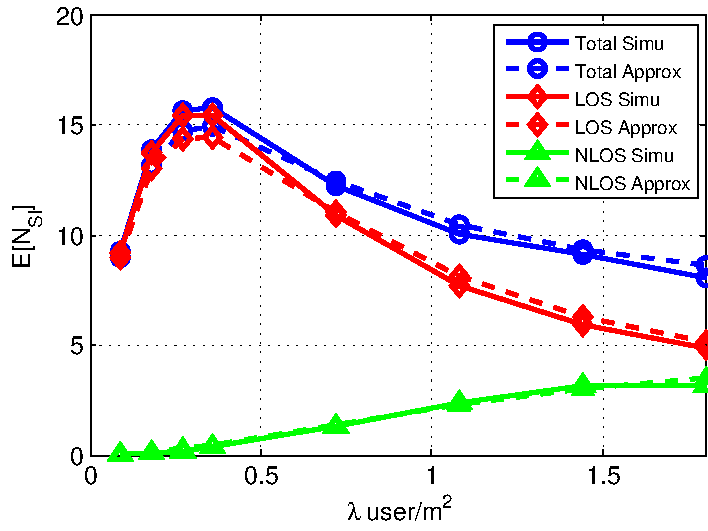
\includegraphics[width = 0.3\textwidth]{Channel_en_si.pdf}
	\caption{$\mathrm{E}[N_{\mathrm{SI}}]$ for different user densities. $h_{\mathrm{body}} = 1.754m$,  $h_{\mathrm{device}}= 1m$, $h_{\mathrm{ceiling}}=2.8m$. 
		The material of the ceiling is one layer polyester board with a thickness of 9 mm. 
		The threshold of path loss for strong interferers is -88 dB, $r_{\max} = 10\mathrm{~m}$, and $r_{\max}^{\mathrm{reflection}} = 3.1m$.}
	\label{fig:channel:en_si}
\end{figure}


\begin{figure}
	\centering
	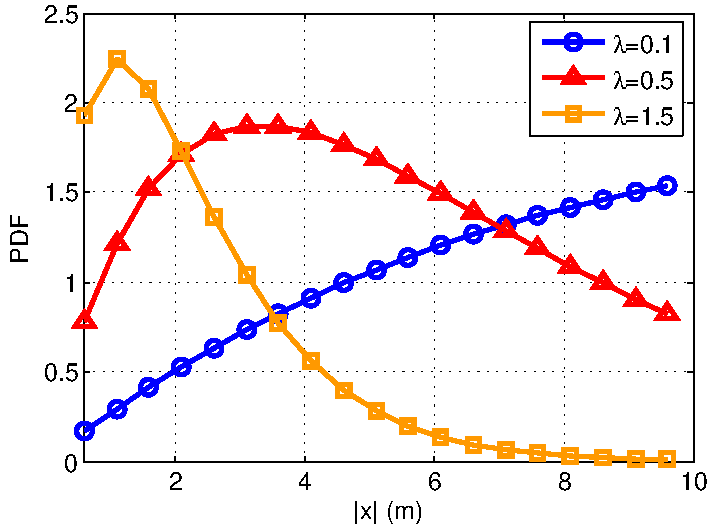
\includegraphics[width = 0.3\textwidth]{Channel_si_pdf.pdf}
	\caption{Probability density function of LOS strong interferers as a function of the distance to the typical user at $0$.}
	\label{fig:Channel_si_pdf}
\end{figure}

\begin{figure}[htp]	
	\centering
	\subfloat[$\lambda = 0.1/m^2$]{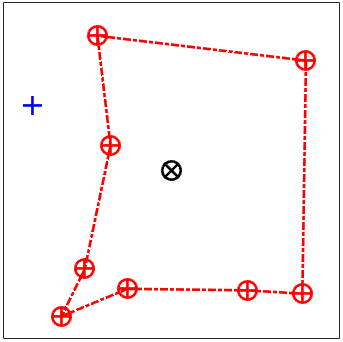
\includegraphics[width=0.15\textwidth]{Channel_jamming_01.pdf}} \hfill
	\subfloat[$\lambda = 0.5/m^2$]{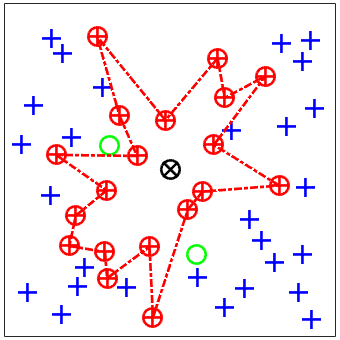
\includegraphics[width=0.15\textwidth]{Channel_jamming_05.pdf}} \hfill
	\subfloat[$\lambda = 1.5/m^2$]{\label{fig:channel:jamming:15} 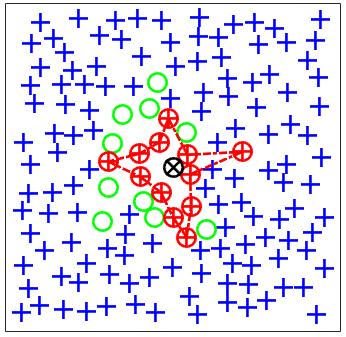
\includegraphics[width=0.15\textwidth]{Channel_jamming_15.pdf}}
	\caption{The locations of strong interferers for different densities, ignoring self blockages. The joint red circles represent LOS interferers, green hollow circles are NLOS interferers and blue crosses are non strong interferers.}
	\label{fig:channel:jamming}
\end{figure}

Fig.~\ref{fig:Channel_si_pdf} illustrates the distribution for the distance of strong interferers for varying user densities. 
Fig.~\ref{fig:channel:jamming} shows the locations of strong interferers in one realization of the network.
As user density increases, the strong interferers tend to concentrate close to the receiver. When user density is very high, the network reaches a ``jamming regime'', where strong interferers are mostly close by and block further away interferers as shown in Fig.~\ref{fig:channel:jamming}\subref{fig:channel:jamming:15}.

%Such results indicate that it might be enough to coordinate close neighboring users.


\subsection{Sensitivity of Strong Interferers}\label{section:channel:sensitivity}
In this section we study the sensitivity of strong interferers to users' small local movements.
The sensitivity of strong interferers, i.e., how the set of strong interferers changes when users move, influences the cost and benefit of tracking and coordinating with such neighbors.

\textbf{Movement model.} 
Suppose in a time interval $[t, t+ \Delta t]$, users make independent small scale movements, i.e., translation $\Delta X_i$ and rotation $\Delta \Theta_i$. 
Denote $\tilde{\Phi}^t$ as the network at time $t$, then the changes for the typical user and potential interferers are summarized as follows:
\begin{equation*}
\begin{split}
(0,\theta_0)&\rightarrow(\Delta x_0, \theta_0 + \Delta\theta_0), \\
\tilde{\phi}^{t}=\{(x_i, \theta_i)\}&\rightarrow\tilde{\phi}^{t+\Delta t}=\{(x_i+\Delta x_i, \theta_i + \Delta\theta_i)\}.
\end{split}
\end{equation*}
%where $\Delta x$ is the translation and $\Delta \theta$ is the angle of rotation, both 
Both $\Delta X$ and $\Delta\Theta$ are identical and independently distributed (i.i.d.), $\Delta X$ is uniformly distributed in $b(0,r_{\mathrm{move}})$, $\Delta \Theta$ is uniformly distributed in $[-\omega, \omega]$.


\textbf{Metric for sensitivity.} Denote $Y_x^t=f_0(x, \theta, \tilde{\phi}^t\backslash (x, \theta), \theta_0)$ as the indicator that user $x$ is a strong interferer at time $t$, and $Y_x^{t+\Delta t}$ as the state of the same user at $t+\Delta t$, i.e.,
\begin{multline*}
Y_{x}^{t+\Delta t} = f_{\Delta x_0}(x+\Delta x, \theta + \Delta\theta, \tilde{\phi}^{t+\Delta t}\backslash (x+\Delta x, \theta + \Delta\theta), \\
\theta_0 + \Delta\theta_0),
\end{multline*}
$Y_x^t \mathrm{~and~} Y_{x}^{t+\Delta t} \in \{0,1\}$.
We define the \emph{sensitivity} of an interferer originally located at $x$ for an interval of length $\Delta t$, $S(x, \Delta t)$, based on the autocorrelation of the state of the interferer at $t$ and $t+\Delta t$ as follows, 
\begin{equation}
S(x, \Delta t)
=\mathrm{Corr}(Y_x^t, Y_x^{t+\Delta t})
=\frac{\mathrm{Cov}(Y_x^t, Y_x^{t+\Delta t})}{\sigma_{Y_x^t}\cdot \sigma_{Y_x^{t+\Delta t}}},
\end{equation}
where $\mathrm{Cov}(Y_x^t, Y_x^{t+\Delta t}) = \mathrm{E}[Y_x^t\cdot Y_x^{t + \Delta t}] - \E[Y_x^t]\E[Y_x^{t+\Delta t}]$, $S(x, \Delta t)\in [0,1]$. If $S(x, \Delta t)$ is small, the autocorrelation between the states of the channel is small and the channel sensitive to movements; if $S(x, \Delta t)$ is close to $1$, the autocorrelation is high and the estimation of interferer is reliable.


\textbf{How to compute \boldmath$S$.}
Based on our assumptions that movements are i.i.d., $\tilde{\Phi}^t$ is stationary (the Displacement Theorem \cite{poisson}).
As a result, 
\begin{gather*}
\sigma_{Y_x^t} = \sigma_{Y_x^{t+\Delta t}}  =\mathrm{P}_{\mathrm{SI}}(x)\cdot (1-\mathrm{P}_{\mathrm{SI}}(x)),\\
\E[Y_x^{t+\Delta t}] \approx \E[Y_x^{t}] = \mathrm{P_{SI}}(x),
\end{gather*}
where $\mathrm{P}_{\mathrm{SI}}(x)=\mathrm{Pr}(f_0(x,\theta,\tilde{\phi}\backslash(x,\theta), \theta_0)=1)$, 
%$\mathrm{E}_{\Delta X, \Delta X_0}[Y_x^{t+\Delta t}] = \E[P_{\mathrm{}}]$ 
and we use $\E[Y_x^{t}]$ to approximate $\E[Y_x^{t+\Delta t}]$. 

$\mathrm{E}[Y_x^t\cdot Y_x^{t + \Delta t}]$ is the probability that user at $x$ is strong interferer at $t$ and $t + \Delta t$,
\begin{equation*}
\mathrm{E}[Y_x^t\cdot Y_x^{t + \Delta t}] = \mathrm{Pr}(\{Y_x^t=1\}\cap \{Y_x^{t+\Delta t}=1\}).
\end{equation*}
User $x$ is a strong interferer at $t$ and $t+\Delta t$ if user $x$ is facing user $0$ and the channel between them is not blocked at $t$ and $t+\Delta t$.
The probability of facing can be computed by taking the expectation over $\Theta_0, \Theta, \Delta \Theta_0, \Delta\Theta$.
Denote $N_\mathrm{B}^{t, t+\Delta t}$ as the number of users blocking the channel between user $x$ and user $0$ at $t$ or $t+\Delta t$. $\tilde{\Phi}^t$ is i.m.p.p. and the movements are i.i.d., thus $N_\mathrm{B}^{t, t+\Delta t}$ follows a Poisson distribution following the Displacement Theorem and $\E[N_\mathrm{B}^{t, t+\Delta t}]$ can be computed using Campbell's formula and the mobility model.


\textbf{Numerical results.}
We present the numerical results on the sensitivity of LOS strong interferers for $\Delta t= 1$s in Fig.~\ref{fig:channel:sensitivity}. 
%$\Delta X$ is uniformly distributed in a disk centered at the origin with the radius of $r(\lambda, \Delta t)$, $\Delta X \sim \mathrm{unif}(b(0, r(\lambda, \Delta t)))$. 
$r_{\mathrm{move}}(\lambda, \Delta t)$ may decrease with user density in dense environment, i.e., 
\begin{equation*}
r(\lambda,\Delta t) = \min(0.23, 0.6 \sqrt{1/\lambda\pi}) \mathrm{~m},
\end{equation*}
We use this model to capture the fact that users' local movements become limited as the distance among users becomes smaller. 
The range for rotation is $48\degree$, i.e., $\omega = 24\degree$. 
Fig.~\ref{fig:channel:sensitivity}\subref{subfig:channel:sensitivity:function} exhibits the sensitivity of users at different distances. 
As can be seen, distant interferers are more sensitive to perturbations than close by interferers. 
This supports the observation that close by users (interferers) will be robust to perturbations and learning the interference from close by neighbors is more reliable. 
Fig.~\ref{fig:channel:sensitivity}\subref{subfig:channel:sensitivity:average} exhibits the average sensitivity of strong interferers $\E[S]$,
\begin{equation*}
\mathrm{E}[S] = \frac{\lambda\int_{\mathbb{R}^2\backslash b(0, r_{\min})}S(x,\Delta t)\cdot \mathrm{P_{SI}}(x) \mathrm{d}x}{\E[N_{\mathrm{SI}}]},
\end{equation*}
for different user densities.
Strong interferers first become more sensitive to movements as $S(x, \Delta t)$ decreases with $\lambda$. 
In highly dense scenarios, strong interferers are closer and the movements become limited, thus the strong interferers become more robust to user local movements.


\begin{figure}
	\centering
	\subfloat[Sensitivity of user $x$]{\label{subfig:channel:sensitivity:function}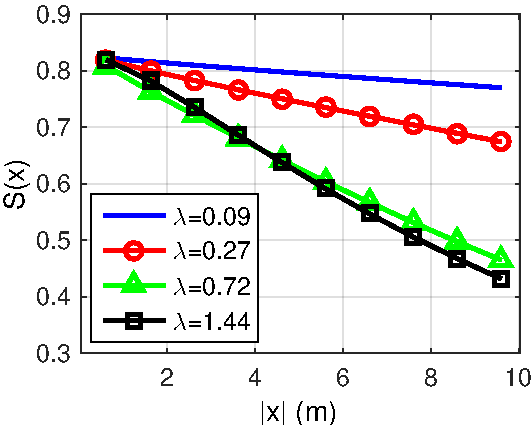
\includegraphics[width=0.23\textwidth]{Channel_sensitivity.pdf} } \hfill
	\subfloat[Average sensitivity]{\label{subfig:channel:sensitivity:average} 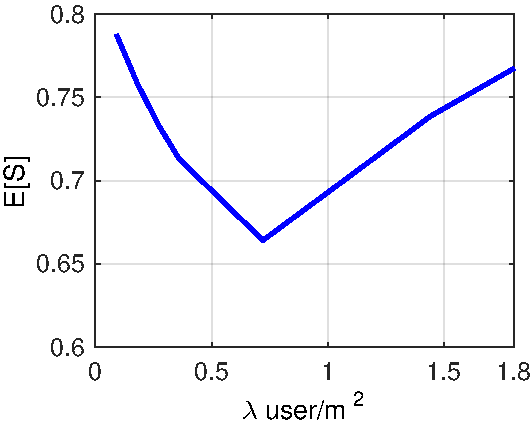
\includegraphics[width=0.23\textwidth]{Channel_sensitivity_average.pdf}}
	
	\caption[]{Sensitivity of users at different distance $|x|$ \subref{subfig:channel:sensitivity:function}, and average sensitivity of strong interferers $\E[S]$ \subref{subfig:channel:sensitivity:average}.}
	\label{fig:channel:sensitivity}
\end{figure}




\section{Optimizing Clustering in Hierarchical Wearable MAC protocols}\label{section:clustering}
In this section, we discuss how to optimize clustering for hierarchical wearable MAC protocols based on our analysis of interference.


\subsection{Hierarchical MAC for Wearable Networks}\label{section:clustering:hierarchy}
When centralized control is absent, hierarchical clustering and scheduling work as a viable solution to coordinating the multiple PBSSs, e.g., the distributed clustering in 802.11ad. 


The hierarchical MAC consists of three parts, clustering, channel selection and scheduling at each PBSS. 
The cluster head synchronizes PBSSs in the cluster and schedules Beacon Transmission Intervals (BTIs) for each cluster member. 
Due to high user density and unstable channels, cluster head may not schedule the data transmissions for cluster members.
Channel selection is mainly used to mitigate interference, either the cluster head select a channel for all members in the cluster, or a PBSS choose the channel to work on then form clusters on that channel. 
Clustering and channel selection help coordinate the PBSSs and are usually performed at a slower time scale. 
In each PBSS, the PCP schedules the data transmissions within the PBSS for each frame while trying to optimize reuse in dense scenarios. 


Current standards leave open the question of how to form clusters and select channels according to the scenario. 
Another major problem is that reuse might be limited, e.g., PBSSs may not use the same slots and work in a time devision multiple access (TDMA) like manner if they can hear other's beacon in 802.11ad.


For dense wearable networks, the basic principle underlying clustering is that the channel between cluster head and cluster members should be strong and stable. 
To better mitigate inter-cluster interference through channel selection, it is also desirable that cluster members share a similar set of strong interferers. 


Based on our analysis of channels, a cluster shall consist of users in close proximity and operate in a channel distinct from that of nearby clusters. 
Apart from applying the above basic principles, one must also choose the proper size for clusters. 
Many factors influence the best cluster size, e.g., channel quality to cluster head, signaling cost, inter-cluster interference, etc. 
We investigate the question by analyzing the impact of cluster size on network reuse. 


\begin{figure}
	\centering
	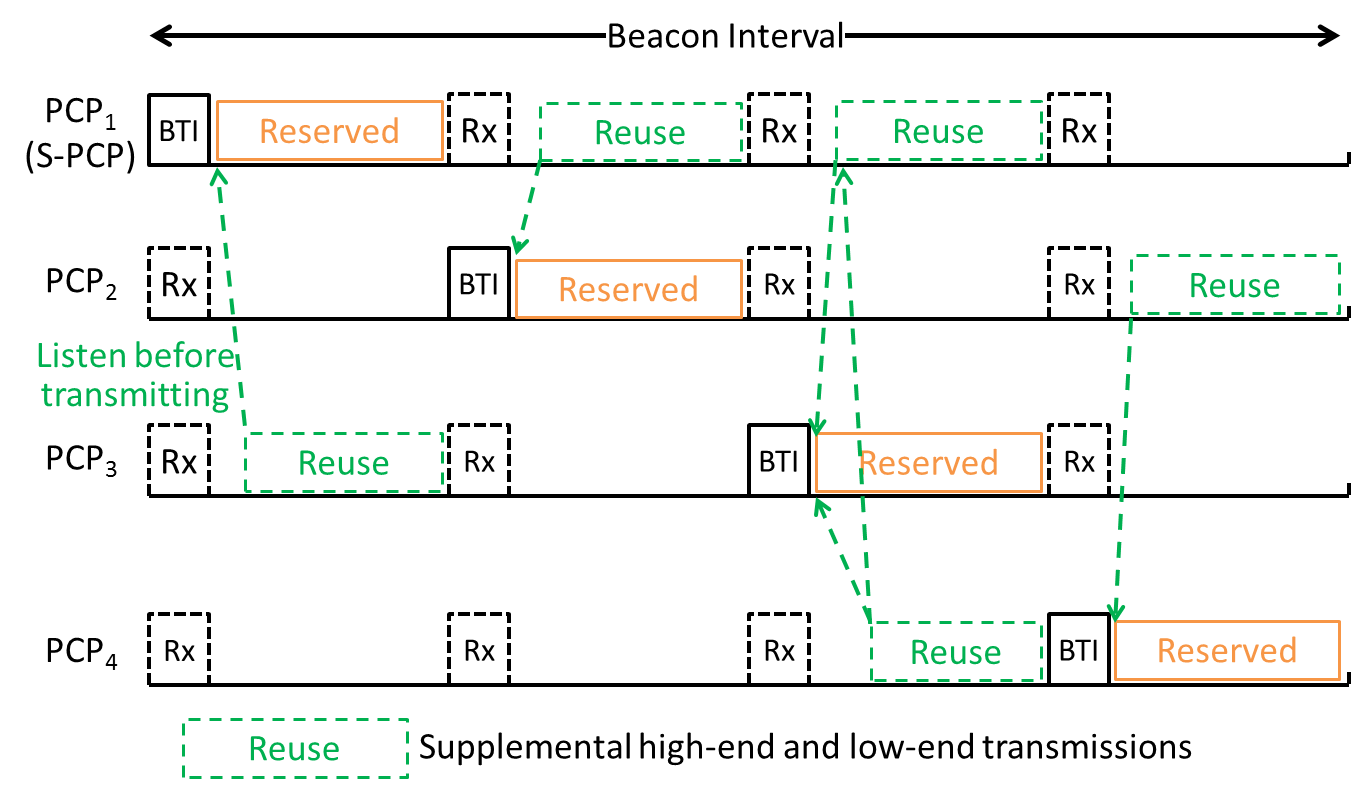
\includegraphics[width = 0.4\textwidth]{Clustering_reuse.pdf}
	\caption{Distributed clustering  with hierarchical scheduling can achieve higher resource reuse and guarantee basic access to channel.}
	\label{fig:clustering:reuse}
\end{figure}


To achieve better resource reuse within the cluster and meet the basic QoS requirements of each PBSS, we propose a hierarchical scheduling method shown in Fig.~\ref{fig:clustering:reuse}. 
Each PBSS is allocated a reserved slot where it has priority over the other PBSSs. 
Other PBSSs may however try to contend with other non-priority PBSSs to reuse slots if the their transmissions do not interfere with the transmissions of the priority PBSS.


\subsection{Modeling Impact of Clustering Size on Achievable Reuse}
In this section we study how cluster size influences the resources made available to each PBSS in a dense wearable networks where clustering and hierarchical scheduling are used. 


Consider the average time that a typical PBSS can perform a successful data transmission, denoted by Successful Transmission Time (STT) as the performance metric of interest.
STT is defined as follows, 
\begin{equation*}
STT = f_{\mathrm{data}}\times p_{\mathrm{access}} \times p_{\mathrm{success}},
\end{equation*}
where $f_{\mathrm{data}}$ is the fraction of time reserved for data transmission, $p_{\mathrm{access}}$ is the probability that the PBSS may access the channel and does not interfere with other PBSSs within the same cluster,
and $p_{\mathrm{success}}$ is the probability that the transmission is free from inter-cluster interference.


There are two types of transmissions, beacon and data transmissions. 
To account for the heterogeneity of devices, e.g., transmission capabilities and QoS requirements, we classify data transmissions of each PBSS into to categories, primary data transmissions with higher priority and highly directional antennas and secondary data transmissions associated with lower priority and less directional antennas. 


\textbf{Modeling clustering and channel selection.}
We assume that clusters are of the same size $K$ and share $M$ channels. Each cluster includes the nearest neighbors of the cluster head and when possible each cluster chooses to operate on different channels than closest neighbor clusters.
In a typical cluster, we model the cluster head as located at the center while the other $K-1$ cluster members are its closest neighbors.
To obtain a tractable simple model, we assume the cluster members are uniformly distributed on a disc centered at the cluster head with a fixed radius $R_{\mathrm{cluster}}$, see Fig.~\ref{fig:clusteranalysis:model}. 
Suppose user density on the disc is the same as $\lambda$, then the expected number of users on the disc should be equal to the number of cluster members, $K - 1$, i.e., 
\begin{equation*}
\lambda \pi (R_{\mathrm{cluster}}^2 - r_{\min}^2) = K - 1,
\end{equation*}
\begin{equation*}
R_{\mathrm{cluster}} = \sqrt{\frac{K - 1}{\lambda\pi}+r_{\min}^2}.
\end{equation*}.

\%Modify this paragraph\%
Channel selection ensures neighboring clusters operate on different channels and form an inter-cluster interference protection region, see Fig.~\ref{fig:clusteranalysis:model}.
Assume the number of clusters on each channel is equal, and all other users operating on the same channel are modeled as uniformly distributed outside the protection region, following a HPPP with density $\lambda/M$.
Assume the number of users in the protection area of each cluster is equal, and protection areas are non-overlapping, then there should be $M\cdot K$ users in the protection area. 
Suppose the user density in the protection region is $\lambda$, then we have 
\begin{equation*}
\lambda \pi (R_{\mathrm{protection}}^2 - r_{\min}^2) = M\cdot K - 1,
\end{equation*}
\begin{equation*}
R_{\mathrm{protect}} = \sqrt{\frac{M\cdot K - 1}{\lambda \pi} + r_{\min}^2}.
\end{equation*}
All users outside the cluster are not synchronized with the cluster and work independently from each other.  

\begin{figure}
	\centering
	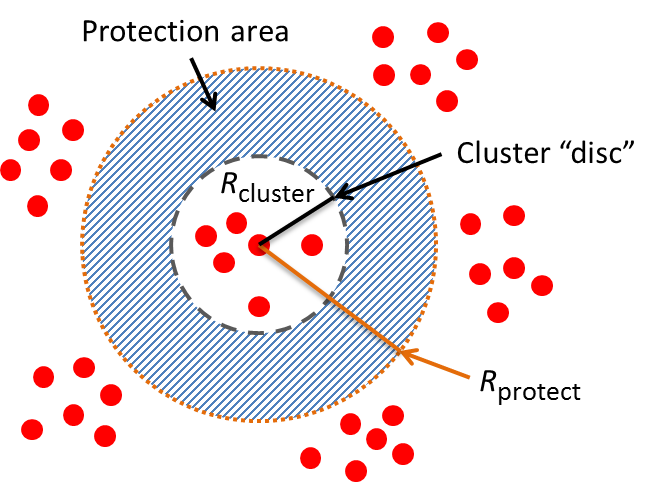
\includegraphics[width = 0.3\textwidth]{Clustering_model.pdf}
	\caption{Model of a typical cluster using clustering and channel selection. Red circles represent users working on the same channel.}
	\label{fig:clusteranalysis:model}
\end{figure}


\textbf{Modeling scheduling.}
%Next we introduce a model for scheduling.
We assume there is at most one transmission in each PBSS in each slot. 
Two transmissions interfere with each other if the received power at either receiver exceeds a threshold.


Let $T_{\mathrm{frame}}$ denote the length of a cluster shared frame and $T_{\mathrm{beacon}}$ the length of one BTI. 
The cluster head reserves exactly $K$ BTIs in $T_{\mathrm{frame}}$ thus the proportion of data reserved for data transmission is given by
\begin{equation*}
f_{\mathrm{data}} = \frac{T_{\mathrm{data}}}{T_{\mathrm{frame}}} = \frac{T_{\mathrm{frame}} - K\cdot T_{\mathrm{beacon}}} {T_{\mathrm{frame}}}.
\end{equation*}
In each BTI, exactly one PCP will transmit its beacon and the other devices will attempt to receive the beacon using omni-directional receive mode. 


The PBSSs are full-buffer and schedule primary transmissions a proportion $\rho_{\mathrm{primary}}\in[0,1]$ of slots for data transmission and schedule secondary transmissions for the remaining $\rho_{\mathrm{secondary}} =1 - \rho_{\mathrm{primary}}$  slots. 


We consider two types of scheduling of transmission within clusters: TDMA and Hierarchical Resource Reuse (HRR). In TDMA scheduling, PBSSs share the slots equally within the cluster and the fraction of time that a PBSS can access the channel in a frame is given by, 
\begin{equation*}
p_{\mathrm{access}}^{\mathrm{TDMA}} = f_{\mathrm{data}}/K.
\end{equation*}
A PBSS schedules primary transmissions in ${\rho_{\mathrm{primary}}f_{\mathrm{data}}}/{K}$ slots, and secondary transmissions in the rest $(1-\rho_{\mathrm{primary}})f_{\mathrm{data}}/K$ slots. 

In HRR, each PBSS is allocated $1/K$ of the slots where it has higher priority. 
The PBSS first schedules primary transmissions in the reserved slots and schedules other transmissions by reusing slots allocated to other PBSSs. 
If $\rho_{\mathrm{primary}}\leq 1/K$, the PBSS also schedules secondary transmissions in the allocated slots. 
Other PBSSs will try to reuse the slots if they do not interfere with the priority PBSS owning the slot.
The probability that a PBSS can reuse a given slot is approximated by
\begin{equation*}
p_{\mathrm{access}}^{\mathrm{HRR}}=(1-\mathrm{P}_{\mathrm{SI}})\cdot \frac{1}{1+\E[N_{\mathrm{intra-cluster}}^{\mathrm{clear}}]},
\end{equation*}
%Discuss how $P_{clear}$ is computed\%
where $\mathrm{P}_{\mathrm{SI}}$ is the probability that the PBSS interfere with the primary PBSS considering the channel path loss and antenna gain,  
%$N_{\mathrm{intra-cluster}}$ is the number of intra-cluster interferers, i.e., PBSSs within the same cluster whose transmissions interferes with the transmission of the typical PBSS.  
$N_{\mathrm{intra-cluster}}^{\mathrm{clear}}$ is number of intra-cluster interferers that are secondary users in the slot and do not interfere with the primary user, i.e., the number of PBSSs contending with the typical PBSS to reuse the slot.



A PBSS's transmission is successful if the transmission is not interfered by transmissions outside the cluster. 
Denote by $N_{\mathrm{inter-cluster}}$ as the number of inter-cluster interfering transmissions. 
The activities of inter-cluster interferers are assumed to be mutually independent thus $N_{\mathrm{inter-cluster}}$ follows a Poisson distribution and the probability of a successful transmission is approximated as follows, 
\begin{equation*}
p_{\mathrm{success}} = e^{-\E[N_{\mathrm{inter-cluster}}]}.
\end{equation*} 
$\E[N_{\mathrm{inter-cluster}}]$ is related to the transmission patterns of PBSSs, which in turn depends on the location of PBSSs within the cluster. 
We use the transmission pattern of a user $\sqrt{2}R_{\mathrm{cluster}}$ away from the cluster head as the typical transmission pattern.

%Validation of mathematical model\%

\subsection{Numerical Results and Discussion}
\%Is the typical user at cluster center good enough?\%
In this section, we compute the achievable STT of the typical user located at the center of the cluster for different scenarios and characterize the cluster size that maximizes the STT. 
The parameters used in our analysis are listed in Table \ref{tab:clusteranalysis:parameter}, the typical user is the cluster head. 

\begin{table}
	\centering
	\caption{The parameters used for numerical analysis}
	\begin{tabular}{cc}
		\hline
		Parameter & Value \\
		\hline
		M & 4 \\
		$h_{\mathrm{ceiling}}$ & 2.8 m \\
		$|\Gamma_{\mathrm{ceiling}}|^2$ & 0.2166 \\
		$\lambda$ & 1 $\mathrm{user/m^2}$ \\
		$P_t^{\mathrm{high}}$ & 10 dBm \\
		$P_t^{\mathrm{low}}$ & 4 dBm \\
		$P_{\mathrm{threshold}}$ & -78 dBm \\
		$\rho_{\mathrm{primary}}$ & 0.5 \\
		$M_t$,$M_r$ ($\theta = 60\degree$) & 5 dB \\
		$m_t$,$m_r$ ($\theta = 60\degree$) & -5 dB \\
		$M_t$,$M_r$ ($\theta = 24\degree$) & 10 dB \\
		$m_t$,$m_r$ ($\theta = 24\degree$) & -10 dB \\		
		$T_{\mathrm{frame}}$ & 100 ms \\
		$T_{\mathrm{beacon}}$ & 2 ms \\
		\hline
	\end{tabular}
	\label{tab:clusteranalysis:parameter}	
\end{table}
% SINR not considered thus don't need noise figure ? 

\textbf{Trade-offs associated with cluster size.} In Fig.~\ref{fig:clusteranalysis:basic} we show how STT and $p_{\mathrm{success}}$ of the typical user vary with cluster size.  
$p_{\mathrm{success}}$ increases with $K$ while $p_{\mathrm{data}}$ and $p_{\mathrm{access}}$ decrease. 
Thus the STT first increases with $K$, then saturates and decreases, indicating that while large clusters may provide good inter-cluster interference mitigation, they increase the contention between users within the same cluster as well as signaling overheads. 
%The STT of primary transmissions is maximized when cluster size is small while the STT of secondary transmissions is maximized for larger $K$, showing that secondary transmissions benefit more from interference mitigation of larger clusters.

\begin{figure}[htp]
	\centering
	\subfloat[Successful transmission time ]{\label{subfig:basic_stt}\includegraphics[width=0.4\textwidth]{Cluster_analysis_basic_stt.pdf} } \hfill
	\subfloat[Probability of successful transmission]{\label{subfig:basic_psuccess} \includegraphics[width=0.4\textwidth]{Cluster_analysis_basic_psuccess.pdf}}
	
	\caption[]{STT for data transmission \subref{subfig:basic_stt} and $p_{\mathrm{success}}$ \subref{subfig:basic_psuccess} for different cluster sizes. $\theta=60\degree$, $\rho_{\mathrm{primary}} = 0.5$. }
	\label{fig:clusteranalysis:basic}
\end{figure}

\textbf{Impact of heterogeneity of devices.} Fig.~\ref{fig:clusteranalysis:primary_ratio} exhibits the STT when users have different proportions of primary transmissions, $\rho_{\mathrm{primary}}$.
As might be expected, the optimal cluster size is smaller when transmissions are more directional. 
Results suggest that highly directional devices are less dependent on clustering to mitigate interference, thus users with highly directional devices may favor small clusters or be better off not joining clusters at all. 


\begin{figure}
	\centering
	\includegraphics[width = 0.3\textwidth]{Cluster_analysis_primary_ratio.pdf}
	\caption{STT for different tranffic patterns $\rho_{\mathrm{primary}}$.}
	\label{fig:clusteranalysis:primary_ratio}
\end{figure}

\textbf{Optimal cluster size v.s. user density.} In Fig.~\ref{fig:clustereanalysis:optimal_cluster_size} we show how the cluster size maximizing the STT changes with user density. 
When user density is high, the optimal cluster size does not change very much, indicating that the optimal cluster size is pretty robust to user density. 
However, as we have discussed, the directionality and proportion of different types of traffic influence the optimal cluster size. 

\begin{figure}
	\centering
	\includegraphics[width = 0.3\textwidth]{Cluster_analysis_optimal_cluster_size.pdf}
	\caption{Cluster size that maximizes STT for different user densities.}
	\label{fig:clustereanalysis:optimal_cluster_size}
\end{figure}

\textbf{STT v.s. user density.} In Fig.~\ref{fig:clusteranalysis:compare_mac} we compare the STT for different MAC protocols and user densities. 
At each user density, the cluster size is chosen as the one that maximizes the STT for the hierarchical MAC with clustering. 
For Aloha, we assume users select channels randomly and the access probability is optimized to maximize the total STT. 
We observe that clustering and reuse provide moderate gains in STT, partly due to beacon overheads. %but can substantially improve the probability of successful transmission. 
We also note that the total STT first decreases with user density then starts to increase with density.
Our result here is different from the existing scaling results on ad hoc networks in that the transmit power or the signal strength does not change with density.
Such a result is in line with our analysis of the interference environment that in very dense networks, close by neighbors block the interference from distant interferers thus the interference in dense environments may not be the worst case. 
 

\begin{figure}
	\centering
	\includegraphics[width = 0.3\textwidth]{Cluster_analysis_compare_mac.pdf}
	\caption{Sum STT in different user densities for different MAC protocols, optimal Aloha, Cluster + TDMA and Cluster + HRR.}
	\label{fig:clusteranalysis:compare_mac}
\end{figure}

%Conclusion for analysis of clusters?


\section{Conclusion}\label{section:conclusion}	
Our analysis of character of interference strong interferers in dense mmWave wearable networks suggests such networks might be quite viable. 
Blockage and directionality help limit the number of strong interferers to a few that are close by and stable.
For a relative stationary network, clustering with resource reuse is a viable solution to coordinating PBSS transmissions. 
Finding the optimal cluster size requires optimizing a trade-off between interference mitigation and resource reuse within clusters thus an ideal cluster protocol should adapt to different environment. 
Our model provide a simple way to explore such trade-offs.


\begin{thebibliography}{50}
\bibitem{wearable}
``Smart Wearable Devices: Fitness, Glasses, Watches, Multimedia, Clothing, Jewellery, Healthcare \& Enterprise 2014-2019,'' \emph{Juniper Research}, Aug. 2014.

\bibitem{80211ad}
\emph{``IEEE Standard for Information Technology — Telecommunications and Information Exchange between Systems — Local and Metropolitan Area Networks — Specific Requirements. Part 11: Wireless MAN Medium Access Control (MAC) and Physical Layer (PHY) Specifications Amendment 3: Enhancements for Very High Throughput in 60 GHz Band,''}, IEEE Standard 802.11ad, 2012.

\bibitem{802153c}
\emph{``IEEE Standard for Information Technology — Telecommunications and Information Exchange between Systems — Local and Metropolitan Area Networks — Specific Requirements. Part 15.3: Wireless Medium Access Control (MAC) and Physical Layer (PHY) Specifications for High Rate Wireless Personal Area Networks (WPANs) Amendment 2: Millimeter-Wave-Based Alternative Physical Layer Extension,''} IEEE Std 802.15.3c, 2009.

\bibitem{ECMA387}
\emph{``High Rate 60 GHz PHY, MAC and PALs,''} ECMA Standard 387, 2010.

%\bibitem{mmwave_propagation}
%S. Y. Geng, J. Kivinen, X. W. Zhao, and P. Vainikainen, ``Millimeter-wave propagation channel characterization for short-range wireless communications,'' \emph{IEEE Trans. Veh. Tachnol.}, vol. 58, no. 1, pp. 3-13, Jan. 2009.

\bibitem{humanshadowing}
C. Gustafson and F. Tufvesson, \emph{``Characterization of 60 GHz Shadowing by Human Bodies and Simple Phantoms, ''} Antennas and Propagation (EUCAP), 6th European Conference on, 2012.

\bibitem{interferencefinitesized}
K. Venugopal, M.C. Valenti and R.W. Heath, \emph{``Interference in Finite-Sized Highly Dense Millimeter Wave Networks,''} Information Theory and Applications Workshop, Feb. 2015.

\bibitem{enclosedmmwave}
G. George and A. Lozano, ``Performance of enclosed mmWave wearable networks,'' in \emph{IEEE Int'l Workshop on Compuational Advances in Multi-Sensor Adaptive Processing (CAMSAP 15)}, Dec. 2015.

\bibitem{urbanblockage}
T. Bai and R.W. Heath Jr., ``Coverage and rate analysis for millimeter wave cellular networks,'' in \emph{IEEE Trans. Wireless Comm.}, vol. 13, no. 9, Sep. 2014.

\bibitem{humanactivity}
S. Collonge, G. Zaharia and G.E. Zein, ``Influence of human activity on wide-band characteristics of the 60 GHz indoor radio channel,'' \emph{IEEE Trans. Wirel. Commun.}, vol. 3,  no. 6, pp. 2369-2406, 2004.

\bibitem{timevaryingpathshadowing}
I. Kashiwagi, T. Taga and T. Imai, ``Time-varying path-shadowing model for indoor populated environments,'' \emph{IEEE Trans. Veh. Technol.}, vol. 59, no. 1, Jan. 2010.

\bibitem{blockagein60ghz}
S. Singh, F. Ziliotto, U. Madhow, E. M. Belding and M. Rodwell, ``Blockage and Directivity in 60 GHz Wireless Personal Area Networks: From Cross-Layer Model to Multihop MAC Design,'' \emph{IEEE J. Sel. Areas Commun.}, vol. 27, no. 8, Oct. 2009.

%\bibitem{virtualtimeslot}
%C. Sum, Z. Lan, R. Funada, J. Wang, T. Baykas, M. A. Rahman, and H. Harada, ``Virtual time-slot allocation scheme for throughput enhancement in a millimeter-wave multi-Gbps WPAN system,'' \emph{IEEE J. Sel. Areas Commun.}, vol. 27, no. 8, Oct. 2009.

%\bibitem{rex}
%L. X. Cai, L. Cai, X. Shen, and J. Mark, ``REX: a randomized exclusive region based scheduling scheme for mmWave WPANs with directional antenna,'' \emph{IEEE Trans Wireless Commun.}, vol. 9, no. 1, pp. 113-121, Jan. 2010. 

%\bibitem{fdmac}
%I. K. Son, S. Mao, M. X. Gong, and Y. Li, ``On frame-based scheduling for directional mmWave WPANs,'' in \emph{Proc. IEEE INFOCOM}, Orlando, FL, 2012, pp. 2149-2157.

\bibitem{dtdmac}
E. Shihab, L. Cai, and J. Pan, ``A distributed asynchronous directional-to-directional MAC protocol for wireless ad hoc networks,'' \emph{IEEE Tans. Veh. Tech.}, vol. 58, no. 9, pp. 5124-5134, Nov. 2009. 

\bibitem{mdmac}
S. Singh, R. Mudumbai, and U. Madhow, ``Distributed coordination with deaf neighbors: efficient medium access for 60 GHz mesh networks,'' in \emph{Proc. IEEE INFOCOM}, San Diego, CA, 2010, pp. 1-9.


\bibitem{intersharing}
W. Feng, Y. Li, D. Jin and L. Zeng, \emph{``Inter-Network Spatial Sharing with Interference Mitigation Based on IEEE 802.11ad WLAN System,''} Globecom 2014 workshop - telecommunications standards - from research to standards


\bibitem{onlinkscheduling}
Z. He, S. Mao and T.S. Rappaport, \emph{``On Link Scheduling Under Blockage and Interference in 60-GHz Ad Hoc Networks,''} edition required...



%\bibitem{mmwaveadhoc}
%A. Thornburg, T. Bai and R.W. Heath Jr., ``Interference statistics in a random mmWave ad hoc network,'' in IEEE Int'l Conference on Acoustics, Speech and Signal Processing (ICASSP), Apr. 2015.

\bibitem{reflection}
K. Sato \emph{et al.}, ``Measurements of Reflection and Transmission Characteristics of Interior Structure of Office Building in the 60-GHz band,'' \emph{IEEE Trans. Antennas Propag.}, vol. 45, no. 12, pp. 1783-1792, Dec. 1997.

\bibitem{poisson}
J. F. C. Kingman, ``Poisson Processes,'' New York: The Clarendon Press Oxford Univ. Press, 1993.

\bibitem{stochasticgeometry}
F. Baccelli and B. Blaszczyszyn, ``Stochastic geometry and wireless networks, volume \Rom{1} - theory,'' \emph{Foundations and Trends in Networking}, vol. 3, no. 3-4, pp. 249-449, 2009.


\bibitem{stochasticapp}
S.N. Chiu, D. Stoyan, W.S. Kendall and J. Mecke, \emph{Stochastic Geometry and its Applications} (3rd ed). Hoboken: Wiley, 2013. 

%\bibitem{busyperiod_heavytraffic}
%P. Hall, ``Heavy Traffic Approximations for Busy Period in an M/G/$\infty$ Queue,'' \emph{Stochastic Processes and their Applications}, vol. 19, no. 2, pp. 259-269, 1985.

%\bibitem{busyperiod_exponential}
%M. A. M. Ferreira and M. Andrade, ``The M/G/$\infty$ Queue Busy Period Distribution Exponentiality,'' \emph{Applimat - Journal of Applied Mathematics}, vol. 4, no. 3, pp. 249-260, 2011.


\bibitem{matern}
B. Mat\'ern, ``Spatial Variation,'' \emph{Lecture Notes in Statistics}, vol. 36, 1986.

%\bibitem{backoff}
%H. Lee, H. Kwon, A. Motskin and  L. Guibas, \emph{``Interference-aware MAC Protocol for Wireless Networks by a Game-Theoretic Approach,''}, in \emph{INFOCOM}, Rio de Janeiro, 2009, pp. 1854-1862.

%\bibitem{apcluster}
%B.J. Frey and D. Dueck, \emph{``Clustering by Passing Messages Between Data Points,''} Science 315 (2007) 972-976.

%\bibitem{apvanet}
%B. Hassanabadi, C. Shea, L. Zhang and S. Valaee, \emph{``Clustering in Vehicular Ad Hoc Networks using Affinity Propagation,''} Ad Hoc Networks 13 (2014) 535-548.

%\bibitem{apd2d}
%D.J. Son, C.H. Yu and D.I Kim, \emph{``Resource Allocation based on Clustering for D2D Communications in Underlaying Cellular Networks,''} in \emph{Information and Communication Technology Convergence}, Busan, 2014, pp. 232-237.


%\bibitem{cocurrentbf}
%J. Qiao, X. Shen, J.W. Mark and Y. He, \emph{``MAC-layer Concurrent Beamforming Protocol for Indoor Millimeter Wave Networks''}, in \emph{IEEE Trans. Veh. Tachnol.}, vol , no. ,   2014. 

\end{thebibliography}

\end{document}
